%% -*- mode: latex; mode: flyspell -*-
\documentclass[12pt, letter]{article}

%% Class name and Assignment number
%%
\newcommand{\courseName}{Introduction~to~Deep~Learning~for~Computer~Vision}
\newcommand{\assignName}{Assignment~4:~PyTorch Classifier I}

%% Packages
\usepackage{amsmath,amsfonts,amssymb,amsthm,dsfont}
\usepackage{graphicx}
\usepackage[bookmarks=false]{hyperref}
\usepackage{color}
\usepackage{float}

%% Paper format
\usepackage{geometry}
\geometry{
    letterpaper,
    %% total={216mm,279mm}, %< NSERC size
    margin=2.00cm,     %< default
    %% margin=1.87cm,       %< NSERC tightest
}

%% Headers and footers
\usepackage[explicit]{titlesec}
\newpagestyle{titlesec_assignment}{
  \sethead{\courseName}{}{\assignName}\setfoot{}{\thepage}{}
  \headrule
  %% \footrule
}

\begin{document}

%% Set header and footer
\pagestyle{titlesec_assignment}

%% Title
\title{\courseName\\\assignName}
\author{Paul Molina-Plant}
\maketitle

\abstract{In this assignment, we implemented a linear classifier using PyTorch
  and visualized the accuracy and loss of our model in Tensorboard.}

\section{Results}

I implemented the classifier by following the specifications and consulting the
appropriate PyTorch documentation. I trained and validated the model on the CIFAR10 dataset
with default config parameters. The final losses and accuracies are highlighted on each plot.
\begin{figure}[H]
  \centering
  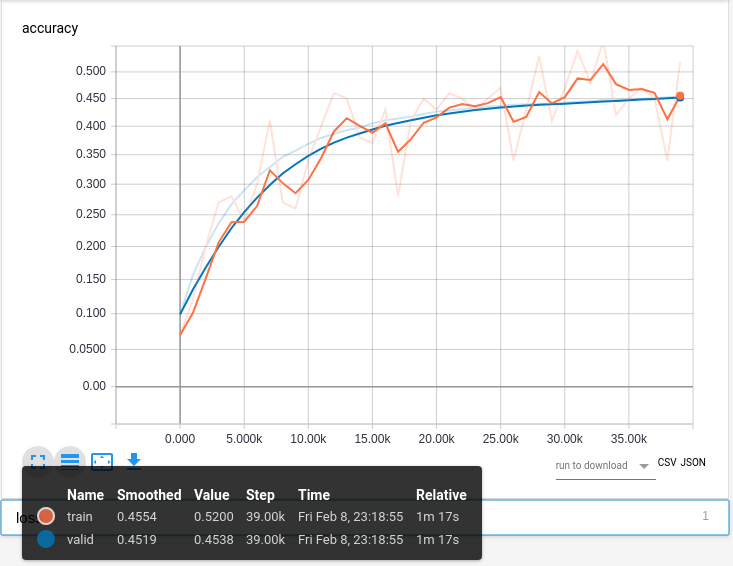
\includegraphics[scale=2.0]{accuracy.png}
  \caption{training and validation accuracy after 100 epochs}
  \label{fig:eg}
\end{figure}
\begin{figure}[H]
  \centering
  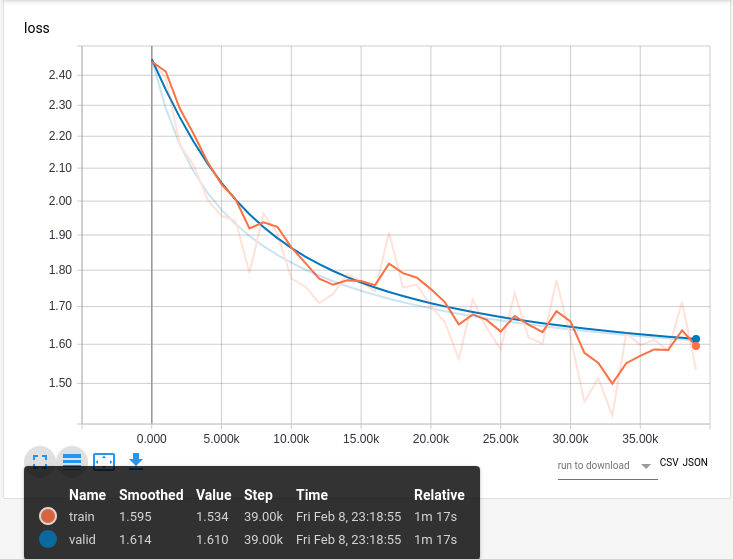
\includegraphics[scale=2.0]{loss.png}
  \caption{training and validation loss after 100 epochs}
  \label{fig:eg}
\end{figure}

\end{document}


%%% Local Variables:
%%% mode: latex
%%% TeX-master: t
%%% End:
